We examine the problem from two perspectives. We present a system based model first and then discuss an agent-based modification of it. We then consider an agent-based model that incorporates agents' movement through space. Throughout the three models we utilize the same assumptions and compartment-state definitions. 

In order to propose a more accurate model and compare the results among different programming  languages, the compartment flow model of the Ebola Epidemic in West Africa, 2014, was modeled with a System Dynamics (SD) and Agent Based Model (ABM) approaches.  Insight Maker and Mathematica was utilized  for the SD, and Insight Maker and Python for the ABM.\\

\begin{itemize}
\item We consider a model of Ebola Outbreak with parameters calibrated for Liberia.
\item We consider two time periods. The first one starts with the announcement of Ebola outbreak in March 2014 and ends the day of the International Intervention in September 2014. The second period covers the time from the International Intervention to July 2015.
\item We ignore all the possible births and deaths occurred due to reasons other that Ebola during the chosen time. 
\item Each individual who dies because of Ebola has a funeral.
\end{itemize}



\subsection{Compartment-State Definition}
Based on the compartmental model and parameters published by Rivers et al.\cite{Rivers2014} in October 2014, it was modeled a similar approach.  This particular model, divides the population into six different compartments; the Susceptible persons (S) could become Exposed (E), if they were in contact with an infected individual, initiating a transition to the Infectious (I) state after the incubation period of the disease, subsequently, acquiring the capacity of infecting others. A percentage of the I class individuals may be Hospitalized (H). There are two possible outcomes for the untreated individuals in I and the treated patients in H, individuals may die, with a probability of infecting other people during the resultant Funeral (F), before the virus is removed (R) from the individual, or the patients may recover, at this stage, can be considered equivalently removed. However,  in order to distinguish between the recovered (R) patients and the deceased (D) individuals, was considered a model with seven compartments : S, E, I, H, F, R and D. Figure ~\ref{fig:compartmentNoFlow} depicts the implemented compartment model. \\


\begin{figure}[!h]
  \centering
  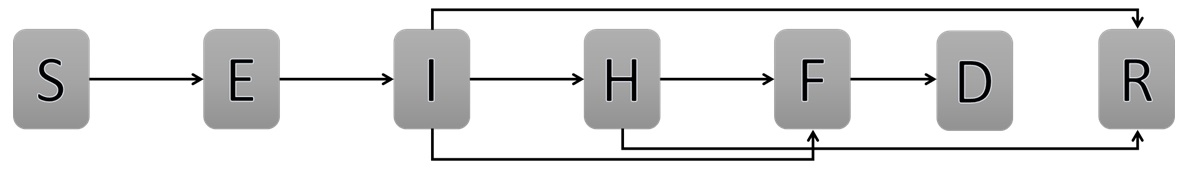
\includegraphics[width=1\textwidth]{compartmentNoFlow}
  \caption{Compartment Model of the Ebola Epidemic in Liberia. \newline  Being S: Susceptible, E: Exposed, I: Infectious, H: Hospitalized, F: Funeral,  R: Recovered and D: Dead.  } 
\label{fig:compartmentNoFlow} 
\end{figure}

\begin{description}
\item[S]- Susceptible. Individuals who have not contracted the disease and have no immunity to it. 
\item[E] - Exposed. Individuals who have come in contact with the Ebola patient and have contracted the disease but do not yet exhibit severe symptoms and thus, are considered not infectious.
\item[I] - Infected. Individuals who experience severe symptoms of Ebola and are contagious.
\item[H] - Hospitalized. Individuals who are infectious and are in the hospital because they are experiencing severe symptoms of Ebola.
\item[F] - Funeral. Diseased but still contagious victims of Ebola. 
\item[D] - Dead. Individuals who died because of Ebola and have been buried. They are considered not to be contagious.
\item[R] - Recovered. Individuals who had Ebola, survived and now are immune to the disease.
\end{description}




\begin{table}[ht]
\caption{Model Parameters for Ebola Epidemic in Liberia.} % title of Table
\centering % used for centering table
\begin{tabular}{c c c}
\hline\hline %inserts double horizontal lines
Parameter & Value  & Reference \\ [0.5ex]
\hline % inserts single horizontal line
Incubation Period (${t_{P}}$) & 11 days & \cite{http : // www.who.int/mediacentre/factsheets/fs103/en/} \\
Duration of Traditional Funeral (${t_{F}}$) & 2.00 days & \cite{Rivers2014} \\
Duration of Infection (${t_{I}}$) & 10.00 days & \cite{Rivers2014} \\
Time from Infection to Death (${t_{D}}$) & 8.00 days & \cite{Rivers2014} \\
Case Fatality Rate, Unhospitalized ($\delta_{1}$) & 0.500 & \cite{http : // www.who.int/mediacentre/factsheets/fs103/en/} \\
Case Fatality Rate, Hospitalized ($\delta_{2}$) & 0.500 & \cite{http : // www.who.int/mediacentre/factsheets/fs103/en/} \\ [1ex]
\hline
\end{tabular}
\label{tab:knownParameters}
\end{table}



